
% utf-8
\documentclass[notes=hide]{beamer}
\usepackage[utf8]{inputenc}
\usepackage[ngerman,english]{babel}
 \usepackage{ngerman}
\usepackage{graphicx}
\usepackage{wasysym}
\usepackage{alltt}
\usepackage{bbm}
\usepackage{stmaryrd}
\usepackage{eurosym}
\usepackage{bm}
\usepackage{xfrac}
\usepackage{hyperref}

\usetheme{uds}

\setbeamerfont{smallfont}{size=\small}
\setbeamerfont{smallerfont}{size=\footnotesize}
\setbeamerfont{smallestfont}{size=\scriptsize}
\setbeamerfont{tinyfont}{size=\tiny}
\setbeamerfont{largefont}{size=\large}
\setbeamerfont{Largefont}{size=\LARGE}

\newcommand\bluebox[2][uds@main]{{%
  \setlength{\fboxsep}{0pt}%
  \colorbox{#1}{#2\strut}%
}}

\def\Prob{\mbox{\bf P}}
\newcommand{\OO}{\mathcal{O}}
\newcommand{\N}{\mathbbm{N}}
\newcommand{\len}[1]{{\vert #1 \vert}}
\newcommand{\emptystring}{\varepsilon}
\newcommand{\substr}[3]{#1[#2\ldots#3]}
\newcommand{\suffix}[2]{{#1}[{#2}\ldots]}
\newcommand{\prefix}[2]{{#1}[\ldots{#2}]}
\newcommand{\chr}[2]{#1[#2]}
\newcommand{\powset}[1]{2^{#1}}
\newcommand{\pos}{\ensuremath{\texttt{\upshape pos}}}
\newcommand{\lcp}{\ensuremath{\texttt{\upshape lcp}}}
\newcommand{\cld}{\ensuremath{\texttt{\upshape cld}}}
\newcommand{\rank}{\ensuremath{\texttt{\upshape rank}}}
\newcommand{\bwt}{\ensuremath{\texttt{\upshape bwt}}}
\newcommand{\bwtfind}{\ensuremath{\texttt{\upshape bwtfind}}}
\newcommand{\Occ}{\ensuremath{\texttt{\upshape Occ}}}
\newcommand{\less}{\ensuremath{\texttt{\upshape less}}}
\newcommand{\type}{\ensuremath{\texttt{\upshape type}}}
\newcommand{\lcpskip}{\ensuremath{\texttt{\upshape skip}}}
\newcommand{\gap}{\ensuremath{\text{--}}}
\newcommand{\iverl}{\llbracket}
\newcommand{\iverr}{\rrbracket}
\newcommand{\C}{\ensuremath{\texttt{\upshape C}}}

\newcommand{\0}{\ensuremath{\mathtt{0}}}
\newcommand{\1}{\ensuremath{\mathtt{1}}}

\newcommand{\rz}{\red\0}
\newcommand{\ro}{\red\1}
\newcommand{\gz}{\green\0}
\newcommand{\go}{\green\1}
\newcommand{\bz}{\blue\0}
\newcommand{\bo}{\blue\1}

\newcommand{\at}{\atopwithdelims..}
\newcommand{\atb}{\atopwithdelims\{\}}
\newcommand{\snp}[2]{\{\blue{#1},\blue{#2}\}}

\newcommand{\mathds}[1]{#1}
\def\cA{\mathcal{A}}
\def\cC{\mathcal{C}}
\def\cN{\mathcal{N}}
\def\cS{\mathcal{S}}
\def\cR{\mathcal{R}}
\def\vG{\mathbf{G}}
\def\vP{\mathbf{P}}
\DeclareMathOperator*{\argmax}{arg\,max}

\newcommand{\blackboard}[1]{
\begin{block}<#1>{}
\begin{center}
\textbf{BLACK BOARD EXAMPLE}
\end{center}
\end{block}
}

\usepackage{listings} % ab Version 1.4 mit Python-Syntax-Highlighting!
\definecolor{mygray}{gray}{.50}
\lstset{language=Python,
    basicstyle=\small\ttfamily,
    stringstyle=\ttfamily\color{green},
    keywordstyle=\color{blue}\bfseries,
    commentstyle=\color{mygray},
    tabsize=4,
    numbers=left,
    numberstyle=\tiny,
    numbersep=5pt,
    morekeywords=assert,
    extendedchars=false,
    showstringspaces=false,
    frame=single
    }
\lstset{escapeinside={/*@}{@*/}}

\newcommand{\captionslide}[1]{
\begin{frame}
\frametitle{\phantom{NONE}}
\begin{center}
\vspace{1cm}
\usebeamerfont{Largefont}
          {\bf\em #1}
          \vspace{2cm}
\end{center}
\end{frame}
}


\title{Day 1: Computational Pan-Genomics:\\Status, Promises and Challenges}
\author[TM]{Erik Garrison and Mikko Rautiainen}
\date{CPANG19 @ Instituto Gulbenkian de Ci\^{e}ncia\\ September, 2019}

\begin{document}

\frame[plain]{\titlepage}

% \begin{frame}{Topics}
% \begin{block}{Past-/Current}
% \begin{itemize}
%  \item long-indel-aware read mapping
%  \item for calling and genotyping structural variations
%  \item for read-based phasing of diploid samples
%  \item for haplotype reconstruction and quantification of virus populations
%  \item for detecting motif-induced sequencing errors in Illumina data
%  \item for calling somatic mutations in cancer.
%  \item GoNL
% \end{itemize}
% \end{block}
% \begin{block}{Current-/Future}
% \begin{itemize}
%  \item Bacterial GWAS
%  \item HGT
% \end{itemize}
% \end{block}
% \end{frame}

\setbeamertemplate{footline}{\hfill\insertframenumber{}\hspace*{10pt}\vskip10pt}

\begin{frame}{Rebooting the Human Genome*}
\textit{"`The Human Genome Project was one of mankind’s greatest triumphs. But the official gene map that resulted in 2003, known as the “reference genome,” is no longer up to the job."'}\\[1em]
(Antonio Regalado, MIT Technology Review, June 3, 2015)\\[5em]

{\scriptsize *\url{https://www.technologyreview.com/s/537916/rebooting-the-human-genome}}
\end{frame}

{ 
\setbeamertemplate{footline}{}
\begin{frame}
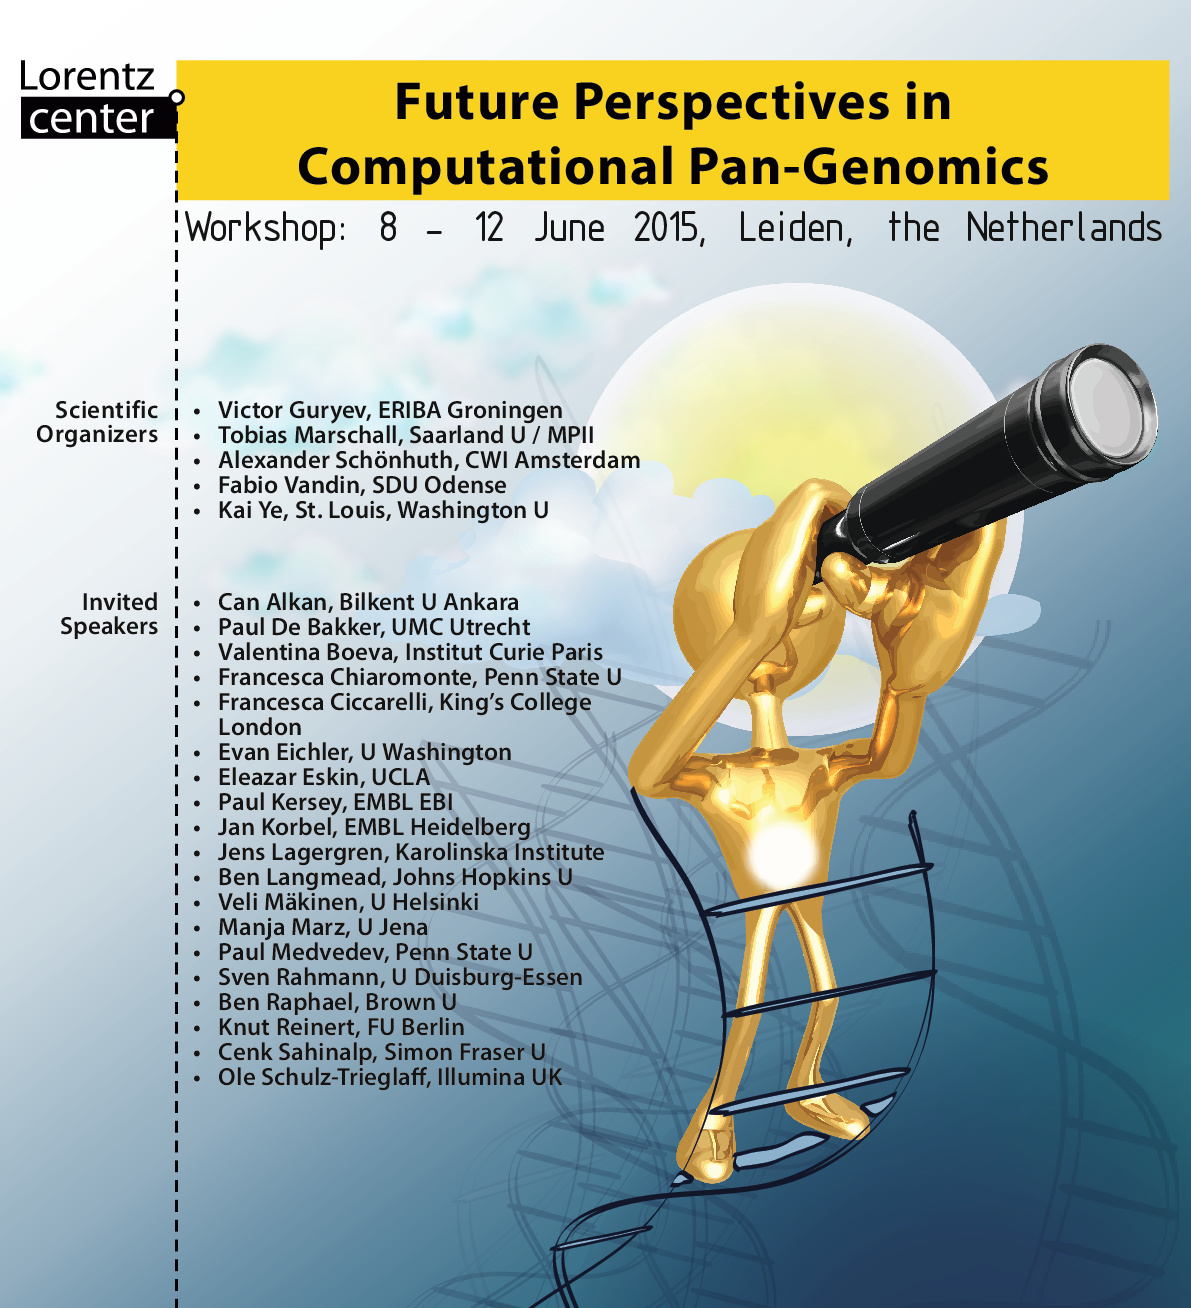
\includegraphics[width=.95\textwidth]{figs/lorentzposter}
\end{frame}
}

{ 
\setbeamertemplate{footline}{}
\begin{frame}{Workshop Paper}
\hspace{1em}
% \\[1em]
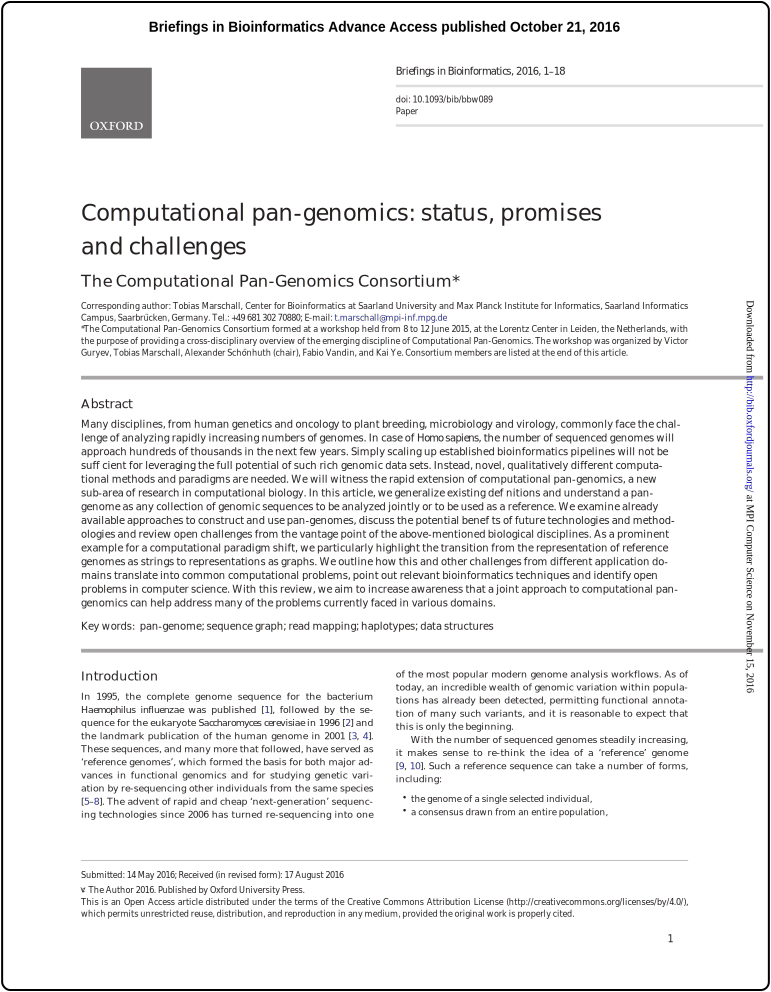
\includegraphics[width=\textwidth]{figs/briefings-paper}
\end{frame}
}

\begin{frame}{Table of Content}
\begin{itemize}
 \item Introduction
 \begin{itemize}
    \item \only<1>{Definition of Computational Pan-Genomics}\only<2>{{\color{red}\textbf{Definition of Computational Pan-Genomics}}}
    \item Goals of Computational Pan-Genomics
 \end{itemize}
\item Applications
 \begin{itemize}
    \item Microbes, Metagenomics, Viruses, Plants, Human Genetic Diseases, Cancer, Phylogenomics
 \end{itemize}
\item Impact of Sequencing Technology on Pan-Genomics
\item Data Structures
 \begin{itemize}
    \item Design Goals
    \item Approaches
 \end{itemize}
\item Computational Challenges
 \begin{itemize}
    \item Read Mapping
    \item Variant Calling and Genotyping
    \item Haplotype Phasing
    \item Visualization
    \item Data Uncertainty Propagation
 \end{itemize}
\end{itemize}
\end{frame}


\begin{frame}[label=pangenomics]{What is a Pan-Genome?}
\begin{block}{}
Term \emph{pan-genome} popularized in microbiology in 2005.
\end{block}
\begin{block}{Definition (gene-based pan-genome)}
The \emph{pan-genome} of a species (or other taxonomic unit) is the \emph{union of all sets of genes} across all individuals.
\end{block}
\uncover<2->{
\begin{center}
\only<1-2>{
\includegraphics[width=\textwidth]{figs/pangenome-flower0}}%
\only<3>{
\includegraphics[width=\textwidth]{figs/pangenome-flower1}}%
\only<4>{
\includegraphics[width=\textwidth]{figs/pangenome-flower2}}%
\end{center}
}
\end{frame}

\begin{frame}{Pan-Genome Definition}
``\textit{... and use the term \emph{pan-genome} to refer to any collection of genomic sequences to be analyzed jointly or to be used as a reference.
These sequences can be linked in a graph-like structure, or simply constitute sets of (aligned or unaligned) sequences.
Questions about efficient data structures, algorithms and statistical methods to perform bioinformatic analyses of pan-genomes give rise to the discipline of \emph{computational pan-genomics}.}''
\begin{block}<2>{Notes}
\begin{itemize}
 \item Not restricted to taxonomic units
 \item Not restricted to full genomes
 \item Not tied to graphs
 \item Intentionally intersects with \emph{metagenomics}, \emph{comparative genomics}, and \emph{population genetics}
\end{itemize}
\end{block}
\end{frame}

% \begin{frame}{Table of Content}
% \begin{itemize}
%  \item Introduction
%  \only<1>{}\only<2>{{\color{red}\textbf{}}}
%  \begin{itemize}
%     \item Definition of Computational Pan-Genomics
%     \item Goals of Computational Pan-Genomics
%  \end{itemize}
% \item Applications
%  \begin{itemize}
%     \item Microbes, Metagenomics, Viruses, Plants, Human Genetic Diseases, Cancer, Phylogenomics
%  \end{itemize}
% \item Impact of Sequencing Technology on Pan-Genomics
% \item Data Structures
%  \begin{itemize}
%     \item Design Goals
%     \item Approaches
%  \end{itemize}
% \item Computational Challenges
%  \begin{itemize}
%     \item Read Mapping
%     \item Variant Calling and Genotyping
%     \item Haplotype Phasing
%     \item Visualization
%     \item Data Uncertainty Propagation
%  \end{itemize}
% \end{itemize}
% \end{frame}

\begin{frame}{Table of Content}
\begin{itemize}
 \item Introduction
 \begin{itemize}
    \item Definition of Computational Pan-Genomics
    \item {\color{red}\textbf{Goals of Computational Pan-Genomics}}
 \end{itemize}
\item Applications
 \begin{itemize}
    \item Microbes, Metagenomics, Viruses, Plants, Human Genetic Diseases, Cancer, Phylogenomics
 \end{itemize}
\item Impact of Sequencing Technology on Pan-Genomics
\item Data Structures
 \begin{itemize}
    \item Design Goals
    \item Approaches
 \end{itemize}
\item Computational Challenges
 \begin{itemize}
    \item Read Mapping
    \item Variant Calling and Genotyping
    \item Haplotype Phasing
    \item Visualization
    \item Data Uncertainty Propagation
 \end{itemize}
\end{itemize}
\end{frame}

\begin{frame}{(High-Level) Goals of Computational Pan-Genomics}
\begin{itemize}
 \item \emph{completeness}: containing all functional elements and enough of the sequence space to serve as a reference for the analysis of additional individuals,
 \item \emph{stability}: having uniquely identifiable features that can be studied by different researchers and at different points in time,
 \item \emph{comprehensibility}: facilitating understanding of the complexities of genome structures across many individuals or species,
 \item \emph{efficiency} organizing data in such a way as to accelerate downstream analysis.
\end{itemize}
\end{frame}

\begin{frame}{Table of Content}
\begin{itemize}
 \item Introduction
 \begin{itemize}
    \item Definition of Computational Pan-Genomics
    \item Goals of Computational Pan-Genomics
 \end{itemize}
\item Applications
 \begin{itemize}
    \item Microbes, Metagenomics, Viruses, Plants, Human Genetic Diseases, Cancer, Phylogenomics
 \end{itemize}
\item Impact of Sequencing Technology on Pan-Genomics
\item Data Structures
 \begin{itemize}
    \item Design Goals
    \item {\color{red}\textbf{Approaches}}
 \end{itemize}
\item Computational Challenges
 \begin{itemize}
    \item Read Mapping
    \item Variant Calling and Genotyping
    \item Haplotype Phasing
    \item Visualization
    \item Data Uncertainty Propagation
 \end{itemize}
\end{itemize}
\end{frame}

\begin{frame}{Approaches I}
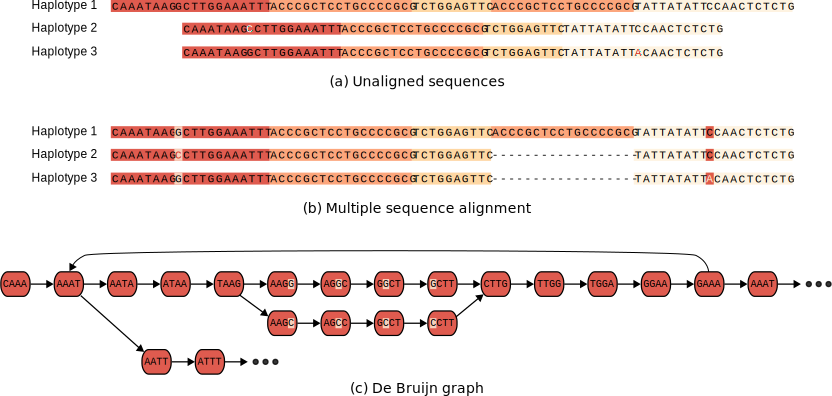
\includegraphics[width=.95\textwidth]{figs/paper/data_structures1}
\end{frame}

\begin{frame}{Approaches II}
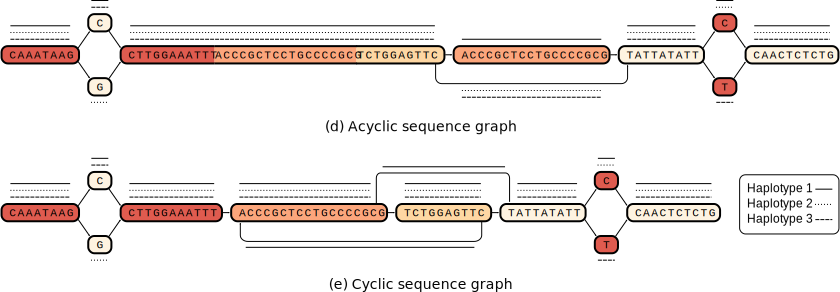
\includegraphics[width=.95\textwidth]{figs/paper/data_structures2}
\end{frame}

\begin{frame}{Approaches III}
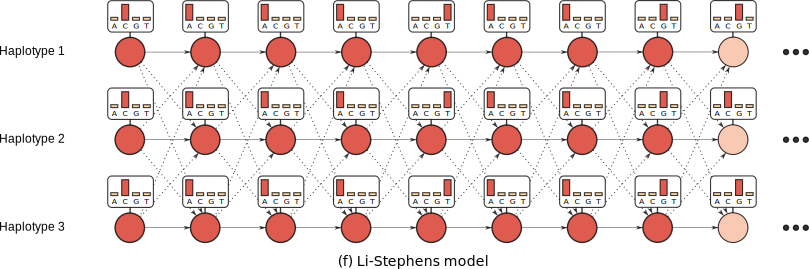
\includegraphics[width=.95\textwidth]{figs/paper/data_structures3}
\end{frame}

\begin{frame}{Course Objectives}
\begin{itemize}
 \item Understand Pan-Genomics concepts and appreciate the \emph{limitations of linear reference genomes},
 \item Learn to build corresponding analysis pipelines in the \emph{VG framework},
 \item We focus on putting you in a position to \emph{design (and debug) pipelines} tailored to your use case,
 \item Some of the practicals address \emph{serious research questions} (that we do not completely solve in class), the aim is rather to give you the tools to attack them.
\end{itemize}
\end{frame}


\begin{frame}{Getting to know each other}
\begin{itemize}
  \item What is your background?
  \item What are your expectations?
  \item Which data / use cases do you work on (or will work on)?
\end{itemize}
\end{frame}

\begin{frame}{Practicals}
\begin{itemize}
 \item This is a hands-on course. We collect praticals in this git repository: \url{https://github.com/Pfern/PANGenomics}
 \item We add new practicals for each day in the course of this week
 \item Ppracticals are a starting point for \emph{exploring what VG can do}. So please don't only copy paste commands, but try to understand their meaning, modify them, etc.
 \item Help each other
 \item Present your results in class
 \item Don't hesitate to send pull requests ;) 
\end{itemize}
\end{frame}


\begin{frame}{Table of Content}
\begin{itemize}
 \item Introduction
 \begin{itemize}
    \item Definition of Computational Pan-Genomics
    \item Goals of Computational Pan-Genomics
 \end{itemize}
\item {\color{red}\textbf{Applications}}
 \begin{itemize}
    \item Microbes, Metagenomics, Viruses, Plants, Human Genetic Diseases, Cancer, Phylogenomics
 \end{itemize}
\item Impact of Sequencing Technology on Pan-Genomics
\item Data Structures
 \begin{itemize}
    \item Design Goals
    \item Approaches
 \end{itemize}
\item Computational Challenges
 \begin{itemize}
    \item Read Mapping
    \item Variant Calling and Genotyping
    \item Haplotype Phasing
    \item Visualization
    \item Data Uncertainty Propagation
 \end{itemize}
\end{itemize}
\end{frame}

\begin{frame}{Applications}
\begin{center}
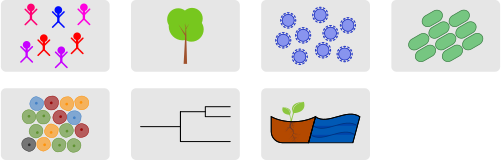
\includegraphics[width=\textwidth]{figs/data-sources}
\end{center}
\end{frame}


\begin{frame}{Application Domain: Microbes}
\begin{itemize}
 \item Pan-genomics at the \emph{gene level}: established workflows and mature software are available
 \item For a number of microorganisms, \emph{pan-genome sequence data is already available}
 \item Microbial pan-genomes support \emph{comparative genomics studies} (especially given horizontal gene exchange)
 \item \emph{Genome-wide association studies (GWAS)} for microbes is an emerging field
\end{itemize}
\begin{center}
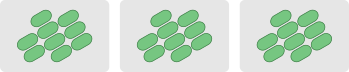
\includegraphics[width=0.8\textwidth]{figs/data-sources-bacteria}
\end{center}
\end{frame}

\begin{frame}{Application Domain: Metagenomics}
\begin{itemize}
 \item Metagenomics: set of genomic sequences \emph{co-occurrence in an environment}
 \item Questions: \emph{taxonomic composition} of the sample, \emph{presence of certain gene products} or whole pathways, and determining \emph{which genomes these functional genes} are associated with.
 \item Pan-Genome data structures present the chance to reveal \emph{common adaptations} to the environment as well as \emph{co-evolution} of interactions.
\end{itemize}
\begin{center}

\includegraphics[width=0.8\textwidth]{figs/data-sources-metagenomics}
\end{center}
\end{frame}

\begin{frame}{Application Domain: Viruses}
\begin{itemize}
 \item Reliable \emph{viral haplotype reconstruction} is not fully solved
 \item \emph{Patient's viral pan-genome} $\rightarrow$ \emph{diagnosis, staging, and therapy selection}
 \item \emph{Virus-host interactions:} pan-genome structure of a viral population to be directly compared with that of a susceptible host population
\end{itemize}
\begin{center}
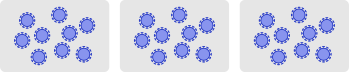
\includegraphics[width=0.8\textwidth]{figs/data-sources-virus}
\end{center}
\end{frame}

\begin{frame}{Application Domain: Plants}
\begin{itemize}
 \item \emph{Large-scale genomics projects} completed / under way: \textit{Arabidopsis thaliana}, rice, maize, sorghum, and tomato
 \item Plant genomes are \emph{large}, \emph{complex} (containing many repeats) and often \emph{polyploid}
 \item Having a pan-genome available for a given crop that includes its wild relatives provides a \emph{single coordinate system} to anchor all known variation and phenotype information
\end{itemize}
\begin{center}

\includegraphics[width=0.8\textwidth]{figs/data-sources-plants}
\end{center}
\end{frame}

\begin{frame}{Application Domain: Human Genetic Diseases}
\begin{itemize}
 \item Numerous genes have been successfully mapped for \emph{rare monogenic diseases}
 \item \emph{Common diseases} $\leftarrow$ GWAS $\leftarrow$ imputation $\leftarrow$ catalogs of human genome variation, their linkage disequilibrium (LD) properties
 \item Pan-Genomics can help to achieve this, especially in \emph{difficult genomic regions}
\end{itemize}
\begin{center}

\includegraphics[width=0.8\textwidth]{figs/data-sources-human}
\end{center}
\end{frame}

\begin{frame}{Application Domain: Cancer}
\begin{itemize}
 \item Improved \emph{detection of somatic mutations}, through improved quality of read mapping to polymorphic regions
%  \item \emph{Somatic cancer pan-genome} ... would enhance the identification of genomic alterations related to the disease (\emph{driver events})
 \item Somatic pan-genome describing the \emph{general somatic variability} in the human population, $\rightarrow$ accurate baseline for assessing the impact of somatic alterations.
 \item Vision: \emph{personal cancer pan-genome} to be built for \emph{each tumor patient}:  single-cell data, haplotype information, sequencing data from circulating tumor cells and DNA, etc.
\end{itemize}
\begin{center}
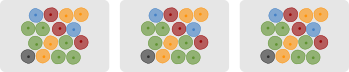
\includegraphics[width=0.8\textwidth]{figs/data-sources-cancer}
\end{center}
\end{frame}

\begin{frame}{Application Domain: Phylogenomics}
\begin{itemize}
 \item Computational pan-genomics: \emph{repidly extrcat evolutionary signals}, such as gene content tables, sequence alignments of shared marker genes, genome-wide SNPs, or internal transcribed spacer (ITS) sequences
 \item Move beyond only using the \emph{best aligned, and most well behaved residues of a multiple sequence alignment} (often used in ``traditional'' phylogenomics)
\end{itemize}
\begin{center}
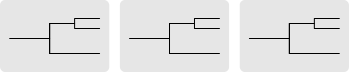
\includegraphics[width=0.8\textwidth]{figs/data-sources-phylo}
\end{center}
\end{frame}

\begin{frame}{Operations on Pan-Genomes}
\begin{center}
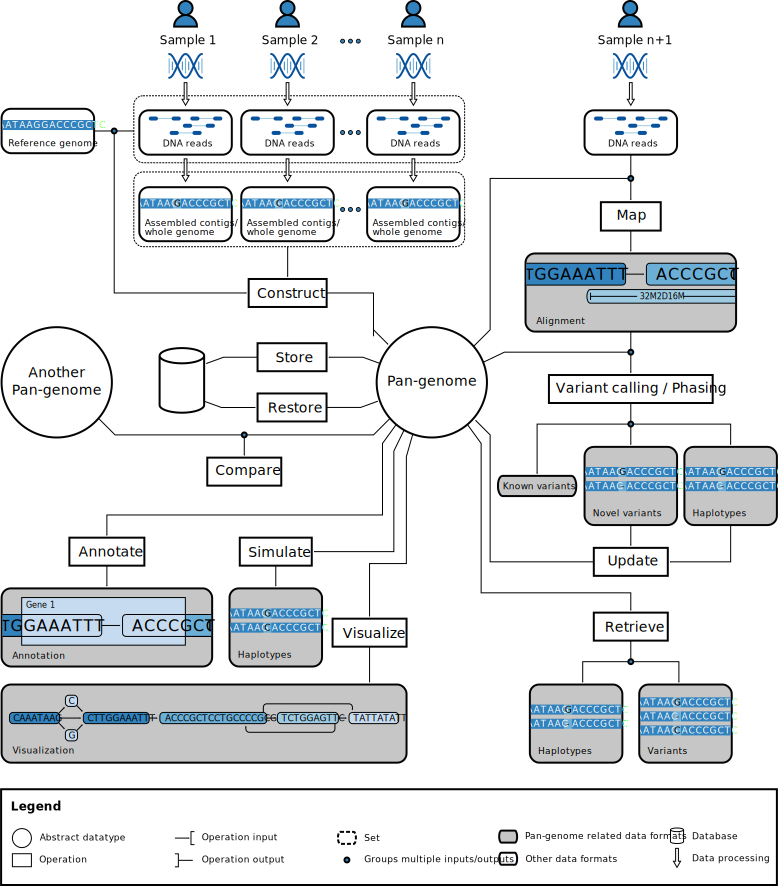
\includegraphics[width=.78\textwidth]{figs/paper/operations}
\end{center}
\end{frame}


\end{document}

\begin{frame}{Table of Content (What I Skipped)}
\begin{itemize}
 \item Introduction
 \begin{itemize}
    \item Definition of Computational Pan-Genomics
    \item Goals of Computational Pan-Genomics
 \end{itemize}
\item Applications
 \begin{itemize}
    \item Microbes, Metagenomics, Viruses, Plants, Human Genetic Diseases, Cancer, Phylogenomics
 \end{itemize}
\item {\color{red}\textbf{Impact of Sequencing Technology on Pan-Genomics}}
\item Data Structures
 \begin{itemize}
    \item Design Goals
    \item Approaches
 \end{itemize}
\item {\color{red}\textbf{Computational Challenges}}
 \begin{itemize}
    \item {\color{red}\textbf{Read Mapping}}
    \item {\color{red}\textbf{Variant Calling and Genotyping}}
    \item {\color{red}\textbf{Haplotype Phasing}}
    \item {\color{red}\textbf{Visualization}}
    \item {\color{red}\textbf{Data Uncertainty Propagation}}
 \end{itemize}
\end{itemize}
\end{frame}


\begin{frame}{Design Goals}
\only<1>{
\textbf{Construction and Maintenance.}\\
Pan-genomes should be constructable from different independent sources, such as
\begin{enumerate}
 \item existing linear reference genomes and their variants,
 \item haplotype reference panels,
 \item raw reads, either from bulk sequencing of complex mixtures or from multiple samples sequenced separately
\end{enumerate}
The data structure should allow \emph{dynamic updates} of stored information without rebuilding the entire data structure, including local modifications such as adding a new genetic variant, insertions of new genomes and deletion of contained genomes
}
 
\only<2>{
\textbf{Coordinate System.}\\
A pan-genome defines the space in which {(pan-)}genomic analyses take place.
It should provide a \emph{coordinate system} to unambiguously identify genetic loci and (potentially nested) genetic variants.
Desirable properties of such a ``coordinate system'' include:
\begin{enumerate}
 \item nearby positions should have similar coordinates
 \item paths representing genomes should correspond to monotonic sequences of coordinates where possible
 \item coordinates should be concise and interpretable
\end{enumerate}
}

\only<3>{
\textbf{Biological Features and Computational Layers.}\\
Annotation of biological features should be coherently provided across all individual genomes.
Computationally these features represent additional layers on top of pan-genomes.
This includes information about
\begin{enumerate}
 \item genes, introns, transcription factor binding sites
 \item epigenetic properties
 \item linkages, including haplotypes
 \item gene regulation
 \item transcriptional units
 \item genomic 3D structure
 \item taxonomy among individuals
\end{enumerate}
}

\only<4>{
\textbf{Data Retrieval.}\\
\begin{itemize}
 \item A pan-genome data structure should provide \emph{positional access to individual genome sequences}, access to all \emph{variants} and to the corresponding \emph{allele frequencies}.
 \item \emph{Haplotypes} should be reconstructable including information about all \emph{maximal blocks and linkage disequilibrium} between two variants.
\end{itemize}
}

\only<5>{
\textbf{Searching within Pan-Genomes.}\\
Comparisons of \emph{short and long sequences (e.g.\ reads)} with the pan-genome ideally results in the corresponding \emph{location and the best matching individual genome{(s)}}.
This scenario may occur for transcriptomic data as well as for DNA re-sequencing data, facilitating the identification of known variants in new samples.
}

\only<6>{
\textbf{Comparison among Pan-Genomes.}\\
Given any pair of genomes within a pan-genome, we expect a data structure to highlight \emph{differences, variable and conserved regions, as well as common syntenic regions}.
Beyond that, a global comparison of two (or more) pan-genomes, e.g.\ with respect to \emph{gene content or population differentiation}, should be supported.
}

\only<7>{
\textbf{Simulation.}\\
A pan-genome data structure should support the generation (sampling) of individual genomes similar to the genomes it contains.
}

\only<8>{
\textbf{Visualization.}\\
All information within a data structure should be easily accessible for human eyes by \emph{visualization} support on \emph{different scales}.
This includes visualization of global genome structure, structural variants on genome level and local variants on nucleotide level, but also biological features and other computational layers should be represented.
}

\only<9>{
\textbf{Efficiency.}\\
We expect a data structure to use as \emph{little space on disk and memory} as possible, while being compatible to computational tools with a \emph{low running time}.
Supporting specialized hardware, such as general purpose graphics processing units (GPGPUs) or field-programmable gate arrays (FPGAs), is partly an implementation detail.
Yet, in some cases, the target platform can influence data structure design significantly.
}

\end{frame}

\begin{frame}{Table of Content (What I Skipped)}
\begin{itemize}
 \item Introduction
 \begin{itemize}
    \item Definition of Computational Pan-Genomics
    \item Goals of Computational Pan-Genomics
 \end{itemize}
\item Applications
 \begin{itemize}
    \item Microbes, Metagenomics, Viruses, Plants, Human Genetic Diseases, Cancer, Phylogenomics
 \end{itemize}
\item {\color{red}\textbf{Impact of Sequencing Technology on Pan-Genomics}}
\item Data Structures
 \begin{itemize}
    \item Design Goals
    \item Approaches
 \end{itemize}
\item {\color{red}\textbf{Computational Challenges}}
 \begin{itemize}
    \item {\color{red}\textbf{Read Mapping}}
    \item {\color{red}\textbf{Variant Calling and Genotyping}}
    \item {\color{red}\textbf{Haplotype Phasing}}
    \item {\color{red}\textbf{Visualization}}
    \item {\color{red}\textbf{Data Uncertainty Propagation}}
 \end{itemize}
\end{itemize}
\end{frame}

\end{document}


